\chapter{Research Methodology}
\label{chap:research-methodoloy}
This chapter presents the research methodology used in this thesis. Firstly, the research motivation is presented in \cref{sec:research-motivation}, followed by the research questions defined for this thesis in \cref{sec:research-questions}. The research method and design are explained in \cref{sec:research-method-and-design}. Then, \cref{sec:design-for-rq1,sec:design-for-rq2} presents the research design for RQ1 and RQ2, respectively. Finally, \cref{sec:technology} presents the various software libraries and hardware used in this thesis.

\section{Research Motivation}
\label{sec:research-motivation}
Writing Smart Contracts are hard. Writing secure Smart Contracts is even harder. Automatic code generation is by many considered the ”holy grail” in the field of computer science \cite{PGL-010}. Ever since OpenAI introduced its first transformer model in the GPT series, this class of transformers has been touted as the state-of-the-art for text generation. Recent works have applied transformers for code generation and program synthesis, achieving state-of-the-art results. For example, Codex by \textcite{chen2021codex} fine-tunes GPT-3 \cite{brown2020language} on code data from GitHub. The results are impressive. However, while the models are improving at a staggering rate, it is also important to consider \textit{how} the models should be used. Works such as \cite{chen2021codex,colin2020pymt5} only consider code synthesis from comments. This is clearly problematic, as users of these systems, developers, do not normally develop code in isolation.

These systems also face many other problems, especially in regards to different biases, for example, gender and security biases. \textcite{chen2021codex} describes that because their model (Codex) is trained on open-source code, including "Public code may contain insecure coding patterns, bugs, or references to outdated APIs or idioms.", the model might "synthesize code that contains these undesirable patterns introduce vulnerabilities" \cite{copilot}. An empirical study by \textcite{pearce2021asleep} found that almost approximately 40\% of the generated code by GitHub Copilot is vulnerable. Security flaws in software can have dire consequences. According to \textcite{smith2020hidden} the estimated cost of cybercrime for 2020 is over \$1 trillion dollars. Due to the monetary nature of blockchain, security flaws are often very severe, as exploits of vulnerabilities often directly result in the loss of funds. One of the most infamous blockchain attacks was the crowdfunding project \acrfull{dao} hack. This hack resulted in an economic loss worth about 60 million dollars at the time \cite{atzei2017asurvey}. Further, the immutable nature prevents the possibility of correcting vulnerable code after being deployed.

This thesis tries to address the problems and limitations described above, by answering the research questions defined in \cref{sec:research-questions}.

\section{Research Questions}
\label{sec:research-questions}
The research questions addressed in this thesis are:

\begin{enumerate}[label=\textbf{RQ\arabic*.}, leftmargin=1.5cm]
    \item How to automatically generate \acrlong{sc} code with transformer-based language models, by inputting comments to guide the code generation?
    \item How to generate secure \acrlong{sc} code with transformer-based language models?
    %\item How to reduce the vulnerability bias in the transformer model.
\end{enumerate}

\section{Research Method and Design}
\label{sec:research-method-and-design}

%The underlying foundation for how research is conducted is rooted in the research philosophy used. For this research, a positivistic research philosophy was used. A positivistic philosophy assumes that the world is not random, that it is ordered and regular, and that one can investigate it objectively. \cite{oates2006researching} A deductive research approach was used. \todo{Remove deductive?}

To best facilitate the answering of the research questions defined in \cref{sec:research-questions}, an \acrfull{dsr} was selected as the research approach. A \acrshort{dsr} focuses on the development and performance of artifacts. For this to be considered research, the work needs to demonstrate academic qualities such as analysis, explanation, argument, justification, and critical evaluation. Further, the work needs to contribute to knowledge in some way \cite{oates2006researching}.
\acrshort{dsr} is typically an iterative process that involves five steps \cite{vaishnavi2004design}: Awareness of Problem, Suggestion, Development, Evaluation, and Conclusion.
\begin{itemize}
    \item \textbf{Awareness of Problem}: is the recognition and formulation of a problem. This might come from multiple sources, such as areas identified by authors for further research, reading about new developments in the industry, from other disciplines, new technological developments, etc. The output of this phase is a proposal for a new research effort, either formal or informal.
    \item \textbf{Suggestion}: directly follows the development of a proposal based on an awareness of a problem. This is the creative step where a tentative idea of how to solve such a problem in a novel way is suggested.
    \item \textbf{Development}: is the actual implementation of the suggested idea. This is the step where the tentative design idea is implemented and produces an artifact. The techniques used for implementation vary with the type of artifact, which could be anything from algorithms to models.
    \item \textbf{Evaluation}: is the evaluation of the artifact. In this step, the artifact's worth is assessed, as well as potential deviations from expectations. 
    \item \textbf{Conclusion}: is the final step where the results from the design process are determined to be "good enough". The results are written up. The knowledge gained is identified, along with any loose ends that might serve as subjects for future research.
\end{itemize}

\noindent
For this thesis, \cref{sec:research-motivation} clearly describes the awareness of the problems this thesis aims to solve. This is the motivation behind the new research effort proposed in this thesis, conveyed as research questions defined in \cref{sec:research-questions}. \cref{sec:design-for-rq1} and \cref{sec:design-for-rq2} describe a suggestion for how to answer these research questions. \cref{chap:implementation-and-results} describes the implementation of the suggested solution for the research questions, while \cref{chap:evaluation} presents an evaluation of the implementation results. Finally, the findings and results are discussed in \cref{chap:discussion}, and areas suitable for further research are presented in \cref{chap:conclusion}.
%
%The next section describes the suggestion step. The next section describes the development step. The next section describes the %evaluation step. The next section describes the conclusion step.
%This thesis aims to solve the research questions defined in \cref{sec:research-questions}. 
%
%These experiments included fine-tuning pre-trained language models, as well as testing these on real data and man-made data. The %results from the evaluation of the fine-tuned models are recorded as observations and quantitatively evaluated.
%
%This project employs . \acrfull{dsr} is a ... 



%The research is conducted objectively. It is based on facts that are repeatable and quantitatively evaluated. 


%Research Philosophy - positivism
%Research Type - inductive (exploratory) + Quantitative
%Research Strategy - experiments (train and test)
%Time Horizon- one-time data set construction (1st of april)
%Sampling Strategy  - probability sampling (random)
%Data Collection Method - Observation? Evaluate performance
%Data Analysis Methods - Employ primarily a quantitative analysis, as well as some qualitative analysis. (mixed methods?)


%\section{Research Implementation}
%\label{sec:research-implementation}
%
%For the implementation of the research, first, the datasets needed for the experiments were constructed. The datasets creation %phase is divided into the following steps:
%\begin{enumerate}
%    \item Create verified smart contract source code dataset.
%    \begin{enumerate}
%        \item Scrape verified smart contracts from the Ethereum blockchain.
%        \item Filter scraped verified smart contracts for uniqueness.
%    \end{enumerate}
%    \item Create an audited version of the smart contract dataset
%    \begin{enumerate}
%        \item Label the smart contracts with a vulnerability detection tool.
%    \end{enumerate}
%    \item Create a parsed dataset containing "comment, function" pairs. This will facilitate testing, as well as research %question 3.
%    \begin{enumerate}
%        \item Create a parser that can parse all contract versions.
%        \item Parsing the verified smart contracts with a parser.
%    \end{enumerate}
%\end{enumerate}
%A comprehensive description of the creation of the datasets used in this project is given in \cref{chap:datasets}.
%\newline
%\newline
%Secondly, the language modeling process is divided into 2 phases:
%\begin{enumerate}
%    \item Fine-tune a transformer model on the verified smart contracts dataset.
%    \item Fine-tune a transformer model on the audited verified smart contract dataset, employing security conditioning.
%\end{enumerate}
%A comprehensive description of the implementation of the language models is given in \cref{chap:language-modeling}.


\section{Design for RQ1}
\label{sec:design-for-rq1}
This section describes the design for research question 1. For constructing a comment-aided system for automatically generating smart contract code, multiple design steps are needed. First, the design for a code comment analysis is described in \cref{sec:code-comments-analysis}. Then the following \cref{sec:language-model} describes the language model selected for use in this thesis. Finally, the design of the fine-tuning process is described in \cref{sec:rq1-fine-tuning-design}

%The project scope in this thesis is limited to the generation of smart contracts for the Ethereum blockchain. 

\subsection{Code comments analysis}
\label{sec:code-comments-analysis}
Code comments come in different shapes and styles. Solidity, the primary \acrshort{sc} language of Ethereum, has no less than 4 different standard comment types. For example, one can use single- or multi-line NatSpec comments. These are comments that can provide rich documentation for functions, return variables and more \cite{natspec}. An example of this is shown in \cref{lst:method-natspec-comment-example}. To provide some insight into how a user can formulate a comment for guiding the code synthesis, a comment analysis is conducted of how these look like in real \acrshort{sc} code. Specifically, a clustering analysis of the comments is conducted. Such an analysis can also be used for providing insight into the performance of the models developed in this project.

\begin{lstlisting}[
    caption={Example of a NatSpec comment.},
    label=lst:method-natspec-comment-example,
    language=Solidity]
/// @title A token implementation
/// @author André Storhaug
/// @notice This is an example implementation
/// @dev All function calls are currently implemented without side effects
\end{lstlisting}

\subsection{Language Model to use}
\label{sec:language-model}
As discussed in \cref{sec:transformers-for-code-synthesis}, there are several available transformer models. However, only a few of them have open-sourced pre-trained weights. Of these, GPT-J \cite{gpt-j} is the largest model that includes code in its pre-training dataset "The Pile", described in \cref{sec:the-pile}. The research community has found these models to outperform existing open-source GPT systems in qualitative programming evaluations \cite{wolf2021}. These findings are further backed by \cite{chen2021codex}. Because of this, the state-of-the-art generative pre-trained transformer model GPT-J is the language model used in this thesis.

\subsubsection{The Pile}
\label{sec:the-pile}
The Pile \cite{gao2021thepile} is an 825 GiB open source dataset for language modeling. The Pile features many disparate domains, including books, GitHub repositories, webpages, chat logs, and medical, physics, math, computer science, and philosophy papers, making it one of the most extensive and diverse datasets available. \cref{fig:treemap-the-pile} shows a treemap of the different parts of the dataset. Especially interesting is that 7.59\% (about 95.16 GiB) of the Pile is made up code from GitHub. Code from around 192K GitHub repositories are included, all with more than 100 stars and smaller than a gigabyte \cite{github-downloader}. Unfortunately, as of February 2022, less than 10 repositories on GitHub contain Solidity code and have over 100 stars \footnote{\url{https://github.com/search?o=desc&q=language\%3ASolidity&type=Repositories}}. Hence there is a need for a dataset made up of \acrshortpl{sc}.

\begin{figure}[htp]
    \centering
    \includegraphics[width=\textwidth]{figures/Treemap-of-Pile-components-by-effective-size.png}
    \caption{Treemap of the Pile components by effective size. Source: \cite{gao2021thepile}}
    \label{fig:treemap-the-pile}
\end{figure}

\subsubsection{Model architecture}
\label{sec:architecture}
Ever since OpenAI introduced its first transformer model in the GPT series, this class of transformers has been touted as the state-of-the-art for text generation. Their latest model, GPT-3 \cite{brown2020language}, is their best performing model with 175 billion parameters. However, the model is not openly available at the current time. GPT-J \cite{gpt-j} with 6 billion parameters (GPT-J-6B) is currently one of the best open-source alternatives to OpenAI's GPT-3. GPT-J was released in June 2021 by EleutherAI \cite{eleutherai}, a grassroots collection of researchers working to open-source AI research. The model is trained on the Pile, an 825 GiB diverse, open-source language modeling data set that consists of 22 smaller, high-quality datasets combined together. See section \cref{sec:the-pile} for a more detailed description of the Pile.

Being a GPT class transformer, GPT-J uses a decoder-only architecture, as can be seen in \cref{fig:gpt-j-architecture}. The GPT-J introduces some notable differences from standard transformer models. Firstly, instead of computing attention and feed-forward layers in sequential order, they are computed in parallel and the results are added together. This decreases communication during distributed training, resulting in increased throughput. Secondly, GPT-J uses \acrfull{rope} \cite{su2021roformer} for position encoding. Opposite to sinusoidal encoding used in standard transformer models (see \cref{sec:embedding-and-positional-encoding}), this is shown to result in better model quality in tasks with long text \cite{su2021roformer}.

\begin{figure}[htbp]
    \centering
    %\def\svgwidth{\linewidth}
    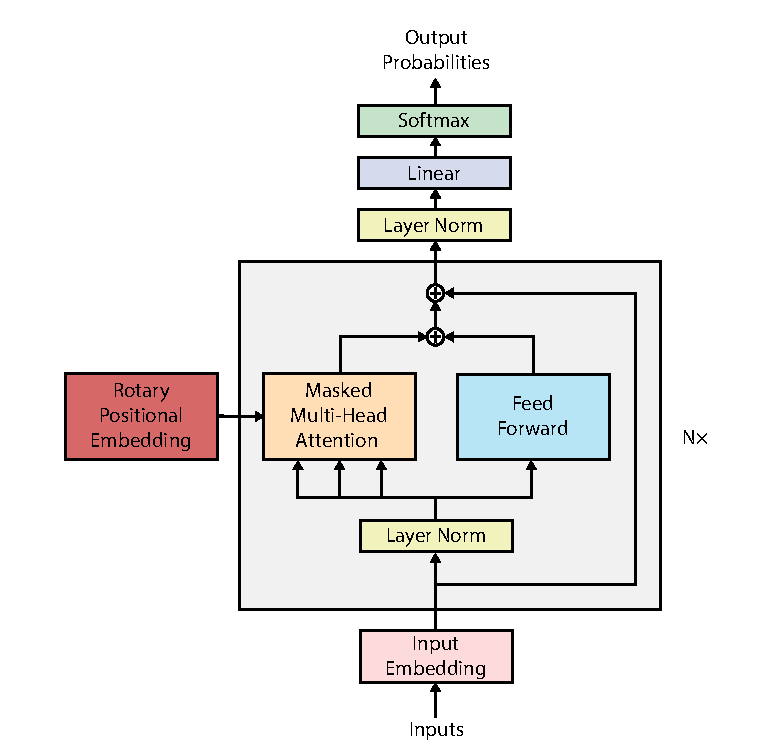
\includegraphics[width=0.8\textwidth]{figures/gpt-j_architecture.pdf}
    \caption{Diagram of GPT-J model architecture.}
    \label{fig:gpt-j-architecture}
\end{figure}

\subsubsection{Requirements}
\label{sec:requirements}
To load the GPT-J model in float32 precision, one would need at least 2x the model size of CPU RAM: 1x for the initial weights and another 1x to load the checkpoint. So for just loading the GPT-J model, it would require at least 48GB of CPU RAM. To reduce the memory footprint, one can load the model in half-precision.

GPU needs around 40GB of GPU memory to load the model. For training/fine-tuning the model, it would require significantly more GPU RAM. For example, the Adam optimizer makes four copies of the model: model, gradients, average and the squared average of gradients. Hence, it would take 4x model size GPU memory, even with mixed precision as gradient updates are in fp32. Further, this doesn't include the activations and data batches which would require some more GPU RAM. Hence, solutions like DeepSpeed \cite{deepspeed} needs to be used for training/fine-tuning such large models.

If a GPU with mixed precision capabilities (architecture Pascal or more recent) is available, one can use mixed precision training with PyTorch 1.6.0 or later, or by installing the Apex library for previous versions. If using an NVIDIA “Ampere” GPU architecture, the \acrfull{bf16} floating-point format can be used. Using mixed precision training usually results in 2x-speedup for training with the same final results.

\subsubsection{Pre-training}
Pre-training is defined as "Training in advance". By first training the model on a huge dataset, the model can then be fine-tuned on a much smaller dataset. This is so-called transfer learning. The pre-training procedure used for GPT class models is called \acrfull{clm} \cite{radford2018improving}. The model reads the text input in order and then tries to predict the next word. The model is fed a complete text element (input sequence) all at once, and then internal masking is applied to prevent the model from cheating by looking at future tokens. For more details on the inner workings of the training procedure, see \cref{sec:transformer-training}.

\subsection{Fine-tuning design}
\label{sec:rq1-fine-tuning-design}
To refine the pre-trained GPT-J-6B model for generating \acrshort{sc} code, the model needs to be fine-tuned on \acrshortpl{sc}. This should allow the model to adapt its existing knowledge gained from the pre-training procedure to produce high-quality \acrshort{sc} code. The fine-tuning procedure used is similar to that of the pre-training procedure. However, instead of using the Pile, a custom dataset of \acrshortpl{sc} needs to be constructed for use. The dataset then needs to be shuffled, before \acrshortpl{sc} are fed to the model for training. To ensure the validity of the model's performance, the dataset used needs to be split into separate sets for training, validation and testing. In this thesis, 80\% of the data will be used for testing, 10\% for validation, and 10\% for testing. After the model is fine-tuned, it should be able to auto-regressively generate \acrshortpl{sc} code. Due to the share size of the selected model (see \cref{sec:requirements}), no hyper-parameter optimization was performed. All hyper-parameters were set to their default values, as used for pre-training.

\section{Design for RQ2}
\label{sec:design-for-rq2}
This section describes the design for research question 2. The proposed method for generating secure \acrshort{sc} code with transformer models is described in \cref{sec:security-conditioning}. Then, the design of the fine-tuning process is described in \cref{sec:rq1-fine-tuning-design}.

\subsection{Security Conditioning}
\label{sec:security-conditioning}
When training a large language model on several gigabytes of open-source code, it is safe to assume that large portions of this code are not safe and contains vulnerabilities. For example, \textcite{durieux2020empirical} analyzed 47.587 real \acrshortpl{sc} with 9 automatic analysis tools. From these, 97\% of the contracts are tagged as vulnerable. This can result in a biased model that may produce a lot of vulnerable code. The idea of this thesis is to use a technique, named security conditioning, to reduce and mitigate this problem. 

The security conditioning is done by prepending a special security label to each of the records in the training data. This way, the model can learn to associate these tokens with either secure or vulnerable code. This way, by also using the labels when generating code, the model may be able to condition whether to produce safe or vulnerable code.

\subsection{Fine-tuning design}
\label{sec:rq2-fine-tuning-design}
For fine-tuning the pre-trained model with security conditioning, much of the same procedure as in \cref{sec:rq1-fine-tuning-design} is used. This makes it possible to validate the technique, by comparing the secured model with the "unsecured" model developed in RQ1. The primary difference is that the dataset records need to be labeled as secure or vulnerable. Before training, the dataset is shuffled and the \acrshortpl{sc} are fed to the model for training. To ensure the validity of the model's performance, the dataset needs to be split into separate sets for training, validation and testing. In this thesis, 80\% of the data will be used for testing, 10\% for validation, and 10\% for testing. To be able to The same hyperparameters used for as in \cref{sec:rq1-fine-tuning-design} no hyper-parameter optimization was performed. All hyper-parameters were set to their default values, as used for pre-training.

After the model is fine-tuned, it should be able to auto-regressively generate \acrshortpl{sc} code. To invoke the security conditioning, one only needs to prepend the security label to the input text.

\section{Technology}
\label{sec:technology}
Following is an overview of the different technologies applied in this project, both software and hardware.

\subsection{Software}
\label{sec:software}
During the selection of the language modeling library for use in this project, several considerations were made. Firstly, due to the huge size of the model, the library needed to support distributed GPU training. It had to be flexible and scalable, without sacrificing too much on speed. The transformers \cite{transformers} library by Hugging Face \cite{huggingface} fulfilled these conditions. The library provides flexible and easy-to-use solutions. It also supports integration with DeepSpeed \cite{deepspeed}, a deep learning optimization library by Microsoft \cite{microsoft} that makes distributed training and inference easy, efficient, and effective. The Hugging Face ecosystem also provides the Datasets and Tokenizers libraries, streamlining and significantly simplifying the use of large datasets.

\paragraph{DeepSpeed}
\label{par:deepspeed}
The deep learning optimization library DeepSpeed \cite{deepspeed} is used for training. It facilitates both distributed training, mixed precision and gradient accumulation, providing significant speedup of the training process while still being able to fit the model into the GPU memory available. The main workhorse of DeepSpeed is the \acrfull{zero} \cite{zero}. \acrshort{zero} comes with three incremental optimization stages: stage 1 (\acrshort{zero}-1), stage 2(\acrshort{zero}-2) and stage 3(\acrshort{zero}-3).

\begin{itemize}
    \item \textbf{Stage 1}: partitions the optimizer states across the processes, so each process only updates its partition.
    \item \textbf{Stage 2}: partitions the reduced gradients for updating the model weights, so that each process only retains the gradients corresponding to its own portion of the optimizer states.
    \item \textbf{Stage 3}: partitions the model parameters across the processes. They are automatically collected and partitioned during forward and backward passes.
\end{itemize}

\noindent
For training exceptionally large models, DeepSpeed also provides heterogeneous memory technologies based on \acrshort{zero}. This includes \acrshort{zero}-Offload for \acrshort{zero}-2 and \acrshort{zero}-Infinity \cite{zeroinfinity} for \acrshort{zero}-3. \acrshort{zero}-Offload offloads the optimizer memory and computation from the GPU to the host CPU. \acrshort{zero}-Infinity is an upgraded version of \acrshort{zero}-Offload that also allows for offloading to \gls{nvme} memory. DeepSpeed \acrshort{zero} makes it possible to train trillion parameter models \cite{zeroinfinity}. However, each optimization stage comes with a performance cost, slowing down the training process. DeepSpeed also provides support for mixed-precision training \cite{mixedprecision}. Mixed-precision training is the use of lower-precision operations (\acrshort{fp16} and \acrshort{bf16}) in a model during training. This both makes it run faster and uses less memory.

\subsection{Hardware resources}
\label{sec:hardware-resources}

The High Performance Computing Platform IDUN \cite{epic} is used for a lot of the tasks in this thesis, especially for the training of the model. IDUN full-fills the requirements defined in \cref{sec:requirements}.

\begin{figure}[htp]
    \centering
    \includegraphics[width=\textwidth]{figures/idun.jpeg}
    \caption{Image of IDUN \cite{idun2}}
    \label{fig:idun}
\end{figure}
